In this section, we present our method to refine \deeppoly{}. \deeppoly{} is a sound and incomplete technique because it does over-approximations. If \deeppoly{} verifies the property then the property is guaranteed to be verified, otherwise, its result is unknown. We overcome this limitation by using a CEGAR-like technique, which is complete. In our refinement approach, we mark some \relu{} neurons to have exact behavior on top of~\deeppoly{} constraints, similar to the strategy of refinement in the most complete state-of-the-art techniques~\cite{wang2021beta,xu2020fast}. We add the encoding of the exact behavior to the~\deeppoly{} constraints and use an \milp{} solver on the extended constraints to check if the extra constraints rule out all spurious counterexamples. The calls to MILP solvers are expensive, therefore we use the spurious counterexamples discovered to identify as small as possible set of marked neurons which suffice to be repaired. %\todo{do we need this para at all? seems repetitive.. move this to intro?}

\subsection{The top level algorithm}
\label{sec:toplevelalgo}
We start by describing Algorithm~\ref{algo:main}, where we present the top-level flow of our approach. The algorithm takes a verification query $\langle N,P,Q \rangle$ as input and returns success if the verification is successful, otherwise returns a counterexample to the query. The algorithm uses supporting algorithms $\textsc{getMarkedNeurons}$ and $\textsc{isVerified}$ (described subsequently) to get more marked neurons to refine and check the validity of the verification query after refinement.

The first line of Algorithm~\ref{algo:main} generates all the abstract constraints by using \deeppoly{}, as described in Section~\ref{sec:deeppoly}. For a node $n_{ij} \in N.neurons$, the abstract constraints consist of the lower and upper constraints as well as the lower and upper bounds. Let $A.lc_i = \Land_{j=1}^{|l_i|} A(n_{ij}).lexpr \leq x_{ij} \leq  A(n_{ij}).uexpr$, which is a conjunction of upper and lower constraints of each neuron of layer $l_i$ with respect to abstract constraint $A$. The $lexpr$ and $uexpr$ for any neuron of a layer contain variables only from the previous layer's neurons, hence $A.lc_i$ contains the variables from layers $l_{i-1}$ and $l_i$. 

\begin{algorithm}[t]
  \textbf{Input: } A verification problem $\langle N,P,Q \rangle$ \\
  \textbf{Output: } UNSAT or SAT
  \begin{algorithmic}[1]
    \State $A := deeppoly(N,P)$\Comment{deeppoly generate the abstract constraints}
    \State marked := \{\}
    \While{True}
      \State result = $\textsc{isVerified}$($\langle N,P,Q \rangle$ , A, marked)
      \If{result = CEX(${v_0}, {v_1} ... {v_k}$)}
        \If{$N({v_0}) \models \lnot Q$}
          \State \textbf{return} Failed(${v_0}$)
        \Else
        \State markedNt := $\textsc{getMarkedNeurons}$($N$ , $A$, $marked$, ${v_0}, {v_1} ... {v_k}$)
          \State marked := marked $\union$ markedNt
        \EndIf
      \Else
        \State \textbf{return} verified
      \EndIf
    \EndWhile
  \end{algorithmic}
  \caption{A CEGAR based approach of neural network verification}
  \label{algo:main}
\end{algorithm}
\begin{algorithm}[t]
  \textbf{Name: } $\textsc{isVerified}$ \\
  \textbf{Input: } Verification query $\langle N,P,Q \rangle$, abstract constraints $A$, and marked $\subseteq ~ N.neurons$ \\
  \textbf{Output: } verified or an abstract counterexample. 
  \begin{algorithmic}[1]
    \State $constr := P \land (\Land_{i=1}^k A.lc_i)\land \neg Q$
    \State $constr := constr \land (\Land_{x \in markedNeurons} exactConstr(x))$ \Comment{as in eq \ref*{eq:reluexact}}
    \State isSat = checkSat(constr)
    \If{isSat}
      \State m := getModel(constr)
      \State \textbf{return} CEX($m(x_0),....,m(x_k)$)
    \Else
      \State \textbf{return} verified
    \EndIf
  \end{algorithmic}
  \caption{Verify $\langle N,P,Q \rangle$ with abstraction A}
  \label{algo:verif1}
\end{algorithm}

\begin{algorithm}[t]
  \textbf{Name: } $\textsc{getMarkedNeurons}$ \\
  \textbf{Input: } Neural network $N$, \deeppoly{} abstraction $A$, $marked\subseteq N.neurons$, and abstract counterexample $({v_0}, {v_1} ... {v_k})$\\
  \textbf{Output: } New marked neurons. 
  \begin{algorithmic}[1]
    % \State \textbf{return} ${x}$ if $N({x}) \models \neg Q$. 
    \State Let ${val^{v_0}_{ij}}$ be the value of $n_{ij}$, when ${v_0}$ is input of $N$. 
    \For{$i=1$ to $k$} \Comment{inputLayer excluded}
      \If{$l_i$ is $\relu${} layer}
        \State $constr := \Land_{t=i}^k A.lc_t$
        \State $constr := constr \land (\Land_{n \in marked} exactConstr(n))$ \Comment{as in eq \ref{eq:reluexact}}
        \State $constr := constr \land \Land_{j=1}^{|l_{i-1}|} (x_{(i-1)j} = val^{v_0}_{(i-1)j})$
        \State $constr := constr \land \Land_{j=1}^{|l_k|} (x_{kj} = v_{kj})$
        \State $softConstrs := \cup_{j=1}^{|l_j|} (x_{ij} = val^{v_0}_{ij})$
        \State $res, softsatSet = \maxsat{}(constr, softConstrs)$ \Comment{res always \sat{}}
        \State $newMarked := \{n_{ij} | 1 \leq j \leq |l_i| \land (x_{ij} = val_i(j)) \notin  softsatSet\}$ 
        \If{$newMarked$ is empty}
          \State \textbf{continue}
        \Else
          \State \textbf{return} newMarked
        \EndIf 
      \EndIf
    \EndFor
  \end{algorithmic}
  \caption{Marked neurons from counterexample}
  \label{algo:refine2}
\end{algorithm}
% \todo{what is N.neurons? should it be Neurons? Answer ashu: N is neural network. N.neurons is the set of neurons}

  
At line 2, we initialize the variable $marked$ to the empty set of neurons.  At the next line, we iterate in a while loop until either we verify the query or find a counterexample. At line 4, we call $\textsc{isVerified}$ with the verification query, abstraction $A$, and the set of marked neurons. In this verification step, the behavior of the marked neurons is encoded exactly, as detailed in Section~\ref{sec:verif}. The call either returns that the query is verified or returns an abstract counterexample, which is defined as follows.

\begin{df}
  A sequence of value vectors ${v_0}, {v_1}, ... , {v_k}$ is an 
  {\em abstract execution} of abstract constraint $A$ if 
  ${v_0} \models lc_0$ and ${v_{i-1}}, {v_i} \models A.lc_i$ for each $i \in [1,k]$.  
  An abstract execution ${v_0,...,v_k}$ is
  an {\em abstract counterexample} if~${v_k} \models \lnot Q$.
\end{df}

If these algorithms return verified, we are done, otherwise we analyze the abstract counterexample $CEX(v_0,...,v_k)$.
At line 6, we first check if executing the neural network $N$ on input $v_0$
violates the predicate $Q$.
If yes, we report input $v_0$ for which the verification query is not true.
Otherwise, we declare the abstract counterexample to be spurious.
We call $\textsc{getMarkedNeurons}$ to analyze the counterexample and
return the cause of spuriousness, which is a set of neurons $markedNt$.
We add the new set $markedNt$ to the old set $marked$ and iterate our loop with the new set of marked neurons. Now let us present $\textsc{isVerified}$ and $\textsc{getMarkedNeurons}$ in detail.

% Algorithm \ref{algo:verif1} exploits the markedNeurons to verify the property. 

%
% The algorithm uses supporting algorithms~\ref{algo:refine1} and~\ref{algo:verif1} to
% verify the query and return either the verification successful or abstractCEX. 

% The algorithm~\ref{algo:main} represents the high-level flow of our approach.



% Our approach contains two parts, the first part contains an approach to finding the markedNeurons. 
% The second part contains the verification approach (utilizing markedNeurons).


% In algorithm ~\ref{algo:refine2} and ~\ref{algo:verif1}
% They are presented in 

% \clearpage

% The goal is to find an input ${x}$, such that the predicates $P({x})$ and 
% $Q(N({x}))$ holds. The predicate $Q$ usually is the negation of the desired property. 
% The triple  is our verification query.
%  \todo{How to formalize $P$ and $Q$}

% An input vector ${v} \in \reals^{|l_0|}$ is a counterexample(cex) if $N({v}) \models \lnot Q$. 
% Let us say $satval_{ij}$ represents the satisfying value of variable $x_{ij}$, after an optimization query. 


% We will use the following convention in writing our algorithms.


% \begin{itemize}
% \item 
% \item 
% % \item $W_i, B_i$ represent the weight and bias matrix of layer $l_i$ respectively. 
% \end{itemize}


% \begin{df}
% \end{df}






\subsection{Verifying query under marked neurons}
\label{sec:verif}
In Algorithm~\ref{algo:verif1}, we present the implementation of 
$\textsc{isVerified}$, which takes the verification query, the \deeppoly{} abstraction $A$,
and a set of marked neurons as input.
At line 1, we construct constraints $contr$ that encodes the executions that satisfy abstraction
$A$ at every step.
At line 2, we also include constraints in $constr$ that encodes the exact behavior of the marked
neurons. The following is the encoding of the exact behavior~\cite{tjeng2017evaluating} of neuron $n_{ij}$.
\begin{align}
    \label{eq:reluexact}
    \begin{split}
      exactConstr(n_{ij}) := x_{(i-1)j} \leq x_{ij} &\leq x_{(i-1)j} - A(n_{(i-1)j}).lb*(1-a) \;\;\land  \\
        0 \leq x_{ij} &\leq A(n_{(i-1)j}).ub*a \land a \in \{0,1\} \\ 
    \end{split}
\end{align}
where $a$ is a fresh variable for each neuron.

At line 3, we call a solver to find a satisfying assignment of the constraints.
If $constr$ is satisfiable, we get a model $m$.
From the model $m$, we extract an abstract counterexample and return it.
If $constr$ is unsatisfiable, we return that the query is verified.


% \subsection{Causes of spuriousness}

% We have a following approach to find the causes of spuriousness (markedNeurons). 

\subsection{Maxsat based approach to find the marked neurons}
\label{sec:markedneurons}
In Algorithm~\ref{algo:refine2}, we present $\textsc{getMarkedNeurons}$
which analyzes an abstract spurious counterexample.
In our abstract constraints, we encode $\affine${} neurons exactly, but
over-approximate $\relu${} neurons.
We identify a set of
marked neurons whose exact encoding will eliminate the counterexample
in the future analysis.
%

As we have also defined earlier, let ${val_i^{{v_0}}}$ represent the value vector
on layer $l_i$, if we execute the neural network on input ${v_0}$.
%
Let us say ${v_0}, {v_1}, ... ,{v_k}$ is an abstract spurious counterexample.
We iterative modify the counterexample such that it becomes more and more
like ${val_i^{{v_0}}}$.
Initially, ${val_0^{{v_0}}}$ is equal to $v_0$.
Since we encode the affine layer exactly in $A.lc_i$, the following
theorem is trivially true.

% % 
% ${v_0}$ is a counterexample if ${val_k^{{v_0}}}$ 
% does not satisfy the property $Q$.

\begin{theorem}
  \label{th:marked2}
  Let us say ${v_0}, {v_1}, ... {v_k}$ is an abstract execution. 
  If $Type_i = \affine$, ${val_i^{{v_0}}} = {v_i}$ if ${val_{i-1}^{{v_0}}} = {v_{i-1}}$.  
\end{theorem}
% \begin{proof}
%   Since affine layer's constraints are exact.
% \end{proof}
% Since $l_0$ is an input layer, so, ${v_0}$ and ${val_0^{v_0}}$ are equal,

By the above theorem, ${v_1}$ and ${val_1^{v_1}}$ are also equal. 
The core idea of our algorithm is to find ${v'_2}$ as close as possible to ${val_2^{v_0}}$, 
such that ${v_0}, {v_1}, {v'_2}, ... {v'_{k-1}}, {v_k}$ becomes an abstract spurious counterexample. 
We measure closeness by the number of elements of ${v'_2}$ are equal to the 
corresponding element of vector ${val_2^{v_0}}$.
\begin{enumerate}
\item If ${v'_2}$ is equal to ${val_2^{v_0}}$ then ${v'_3}$ will also become 
  equal to ${val_3^{v_0}}$ due to theorem \ref{th:marked2}. 
  Now we move on to the next $\relu${} layer $l_4$ and try to find the similar point ${v'_4}$, such that 
  ${v_0}, {v_1}, {v_2}, {v_3},{v''_4}... {v''_{k-1}},{v_k}$ is an . 
  We repeat this process until the following case occurs. 
\item If at some $i$, we can not make ${v'_i}$ equal to ${val_i^{v_0}}$ then we collect the neurons
  whose values are different in ${v'_i}$ and ${val_i^{v_0}}$. We call them marked neurons.
\end{enumerate}

In the algorithm, the above description is implemented using \maxsat{} solver.
The loop at line 2 iterates over $\relu${}~layers.
In lines 4-7, we build constraints that encode that from layer $i$ onward
\deeppoly~abstract constraints are satisfied,
the marked neurons have exact behavior, layer $(i-1)$ neurons have value equal to
${val_{i-1}^{v_0}}$, and the execution finishes at $v_k$.
At line 8, we construct soft constraints $softConstrs$, which encodes $x_{ij}$ is equal to $val_{i}^{v_0}$.
At line 9, we call \maxsat{} solver. 
This call to \maxsat{} solver will always find a satisfying assignment because
our hard constraints are always satisfiable.
The solver will also return a subset $softsatSet$ of the soft constraints.
At line 10, we check which soft constraints are missing in $softsatSet$.
The corresponding neurons are added in $newMarked$.
If $newMarked$ is empty, we have managed to find a spurious
abstract counterexample from $val^{v_0}_{i}$.
We need to go to the next layer.
Otherwise, we return the new set of marked neurons.

%% \begin{figure}
%%   \centering
%%   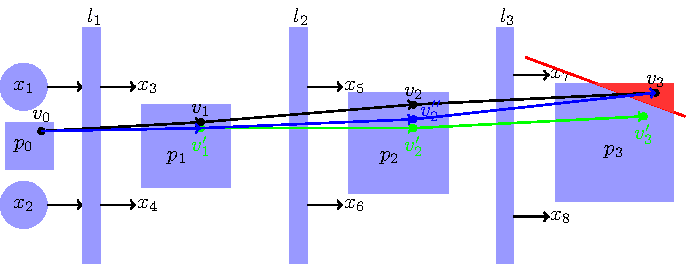
\includegraphics[scale=0.55]{fig/pictorial2.pdf}
%%   \caption{Pictorial representation of our approach}
%%   \label{fig:pictorial}
%% \end{figure}

% \subsection{Utilizing of spurious information}
% The \emph{isVerified} function in algorithm~\ref{algo:main} calls algorithm~\ref{algo:verif1}. 
% The algorithm~\ref{algo:verif1} takes \markednewrons{} as input. 
% The \markednewrons{} represent the set of the culprit neurons. 
% Algorithm~\ref{algo:verif1} replaces the abstract constraints of \markednewrons{} by exact constraints and check for the 
% property by \milp{} solver. If \milp{} solver return \sat{} then we return satisfying assignments as an abstractCEX, 
% otherwise, return verified. 
















%--------------------- DO NOT ERASE BELOW THIS LINE --------------------------

%%% Local Variables:
%%% mode: latex
%%% TeX-master: "../main"
%%% End:

